% !TEX program = pdflatex
% latex-ops example: research article + Minimal Research preset.
% Prompt: "Short note on the convergence rate of gradient descent on strongly convex quadratics,
% with a theorem, the algorithm, a figure and a table. pdfLaTeX, no venue."
% Every number in the figure and table follows from the stated formulas; nothing is measured or invented.
\documentclass[11pt,a4paper]{article}

\usepackage[english]{babel}
\usepackage[T1]{fontenc}
\usepackage{microtype}
\usepackage[a4paper,margin=27mm]{geometry}
\usepackage{amsmath,mathtools,amsthm} % amsthm must precede newtxmath
\usepackage{newtxtext,newtxmath}
\usepackage{booktabs}
\usepackage{siunitx}
\usepackage{pgfplots}
\pgfplotsset{compat=1.18}
\usepackage{algorithm,algpseudocode}
\usepackage[font=small,labelfont=bf]{caption}
\usepackage[hidelinks]{hyperref}
\usepackage[capitalise,noabbrev]{cleveref}

\newtheorem{theorem}{Theorem}
\theoremstyle{definition}
\newtheorem{definition}{Definition}
\DeclarePairedDelimiter{\norm}{\lVert}{\rVert}
\newcommand{\R}{\mathbb{R}}
\widowpenalty=10000 \clubpenalty=10000

\title{\vspace{-2em}A Short Note on Gradient Descent\\for Strongly Convex Quadratics}
\author{A.\ Example\thanks{Illustrative example generated with latex-ops.}}
\date{October 2026}

\begin{document}
\maketitle

\begin{abstract}
\noindent We restate the classical linear convergence result for gradient descent on
strongly convex quadratic functions, give the optimal constant step size, and show how the
number of iterations grows with the condition number. The aim is a compact, self-contained
reference with the proof, the algorithm and the resulting iteration counts.
\end{abstract}

\section{Setting}

Let $f(x) = \tfrac12 x^\top A x - b^\top x$ with $A \in \R^{n\times n}$ symmetric and
\begin{equation}\label{eq:spectrum}
  \mu I \preceq A \preceq L I, \qquad 0 < \mu \le L .
\end{equation}

\begin{definition}
The \emph{condition number} of $f$ is $\kappa = L/\mu \ge 1$.
\end{definition}

The unique minimiser is $x^\star = A^{-1}b$. Gradient descent with constant step
$\eta > 0$ is \cref{alg:gd}.

\begin{algorithm}[ht]
\caption{Gradient descent with constant step}\label{alg:gd}
\begin{algorithmic}[1]
\Require $x_0 \in \R^n$, step $\eta > 0$, tolerance $\varepsilon > 0$
\State $k \gets 0$
\While{$\norm{\nabla f(x_k)} > \varepsilon$}
  \State $x_{k+1} \gets x_k - \eta\,(A x_k - b)$
  \State $k \gets k + 1$
\EndWhile
\State \Return $x_k$
\end{algorithmic}
\end{algorithm}

\section{Convergence}

\begin{theorem}\label{thm:rate}
Under \eqref{eq:spectrum}, the step $\eta = 2/(L+\mu)$ gives
\begin{equation}\label{eq:rate}
  \norm{x_k - x^\star} \le \left(\frac{\kappa - 1}{\kappa + 1}\right)^{k} \norm{x_0 - x^\star}.
\end{equation}
\end{theorem}

\begin{proof}
Since $\nabla f(x^\star) = 0$, the error $e_k = x_k - x^\star$ satisfies
$e_{k+1} = (I - \eta A)\, e_k$. The eigenvalues of $I - \eta A$ are $1 - \eta\lambda$
with $\lambda \in [\mu, L]$, so
$\norm{e_{k+1}} \le \max_{\lambda \in [\mu, L]} \lvert 1 - \eta\lambda \rvert \, \norm{e_k}$.
The maximum is minimised when $1 - \eta\mu = -(1 - \eta L)$, that is
$\eta = 2/(L+\mu)$, where it equals $(L-\mu)/(L+\mu) = (\kappa-1)/(\kappa+1)$.
Induction on $k$ gives \eqref{eq:rate}.
\end{proof}

\section{Iteration counts}

By \eqref{eq:rate}, reducing the error by a factor $10^{-6}$ takes the smallest $k$ with
$\bigl((\kappa-1)/(\kappa+1)\bigr)^{k} \le 10^{-6}$. \Cref{fig:rate} plots the bound and
\cref{tab:iters} lists the counts; for large $\kappa$ they approach
$\tfrac{\kappa}{2}\ln 10^{6}$, linear in the condition number.

\begin{figure}[ht]
\centering
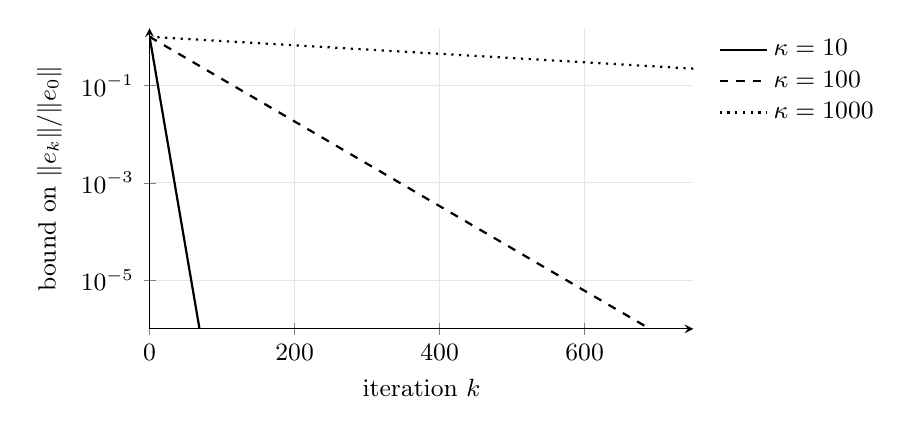
\begin{tikzpicture}
\begin{semilogyaxis}[
  width=0.7\linewidth, height=5.4cm,
  xlabel={iteration $k$}, ylabel={bound on $\norm{e_k}/\norm{e_0}$},
  xmin=0, xmax=750, ymin=1e-6, ymax=1.5,
  legend pos=outer north east, legend cell align=left,
  tick label style={font=\small}, label style={font=\small}, legend style={font=\small, draw=none},
  axis lines=left, grid=major, grid style={gray!20},
]
\addplot[black, thick, domain=0:750, samples=300] {(9/11)^x};
\addlegendentry{$\kappa = 10$}
\addplot[black, thick, dashed, domain=0:750, samples=300] {(99/101)^x};
\addlegendentry{$\kappa = 100$}
\addplot[black, thick, dotted, domain=0:750, samples=300] {(999/1001)^x};
\addlegendentry{$\kappa = 1000$}
\end{semilogyaxis}
\end{tikzpicture}
\caption{The bound \eqref{eq:rate} for three condition numbers. Line style, not colour,
distinguishes the curves, so the figure survives grayscale printing.}
\label{fig:rate}
\end{figure}

\begin{table}[ht]
\centering
\caption{Iterations needed to reduce the error by $10^{-6}$ with $\eta = 2/(L+\mu)$.}
\label{tab:iters}
\begin{tabular}{S[table-format=4.0] S[table-format=1.4] S[table-format=4.0] S[table-format=4.0]}
\toprule
{$\kappa$} & {rate $(\kappa-1)/(\kappa+1)$} & {iterations} & {$\lceil \tfrac{\kappa}{2}\ln 10^6 \rceil$} \\
\midrule
10   & 0.8182 & 69   & 70   \\
100  & 0.9802 & 691  & 691  \\
1000 & 0.9980 & 6908 & 6908 \\
\bottomrule
\end{tabular}
\end{table}

\section{Remarks}

The bound is tight for quadratics: an initial error along the eigenvectors of $\mu$ or $L$
attains it. Methods with momentum improve the dependence from $\kappa$ to $\sqrt{\kappa}$;
that comparison is outside the scope of this note.

\end{document}
